
\documentclass[crop]{CSLB}%%%% Modified CSL template tom include Bibliography



\usepackage{amsmath} %for dealing with mathematics,
\usepackage{amsthm} %for dealing with theorem environments,
\usepackage{cite} %%%for dealing with citations
\usepackage{hyperref} %for linking the cross references
\usepackage{graphics} %for dealing with figures.
\usepackage{algorithmic} %for describing algorithms
\usepackage{subfig} %for getting the subfigures e.g., "Figure 1a and 1b" etc.
\usepackage{url} %It provides better support for handling and breaking URLs.




\jname{International Journal of Astrobiology}%

\newtheorem{theorem}{Theorem}
\newtheorem{condition}{Condition}

\begin{document}

\supertitle{Research Paper}

\title[Probabilities of SETI contacts]{Probability of causal
contact between interstellar civilizations through MonteCarlo simulations}

\author[verso running head]{Lares M$^{1, 2}$, Funes J$^{1, 3}$}

\corres{\name{Lares M} \email{marcelo.lares@unc.edu.ar}}

\address{
   %
   \add{1}{CONICET, Argentina}
   
   \add{2}{Universidad Nacional de C\'ordoba, Observatorio
   Astron\'omico de C\'ordoba, Argentina}
   
   \add{3}{Universidad Cat\'olica de C\'ordoba, Argentina}
   %
}

\begin{abstract}
%
The abundance of intelligent civilizations in the galaxy is a
longstanding question, which is often conceptualized as the problem
of the lack of received communication of the Fermi paradox.
%
Most efforts on the estimation of a number of intelligent
civilizations are centered on the Drake equation, although 
its factors are affected by large uncertainties, and it lacks a
temporal nature.
%
Here we present numerical simulations of stochastic processes of
emergence of civilizations with communication capabilities, and
the causal contacts among them.
%
We analyze the rate of causal contacts as a function of the mean
number of civilizations and the mean lifetime span distribution.
%
Our results indicate that, given the large distances involved, in
the odds to obtain a contact in a few years of monitoring, assuming a
perfect detection rate, are very rare.                                 
%
\end{abstract}

\selfcitation{Lares M, Funes J (XXXX).  Estimating the probability of
causal contact between civilizations through MonteCarlo simulations,
International Journal of Astrobiology}

\received{xx xxxx xxxx}
\revised{xx xxxx xxxx}
\accepted{xx xxxx xxxx}

\keywords{SETI, Computer simulations, Statistics}

\JELclassification{XX; XX}
\MSCcodes{XX; XX}

\Abbreviations{CETI: Communicating Extraterrestrial Intelligence, DE:
Discrete Event, GHZ: Galactic Habitable Zone}

\maketitle

\Fpagebreak

\section{Motivations: Uncertainties and the non detection problem for
ETI contact}
%{{{

A common approach to discuss the possible number of extraterrestrial
intelligent civilizations (ETI) has been the use of the Drake equation
\citep{Gleiser2010, Prantzos2013, Haqq-Misra2017}.
%
However, the uncertainties in the factors make it less prone to a
formal application to define searching strategies or to compute
actual numbers, but is used to organize the discussion instead.
%
Some modifications to the original idea of the equation have tried to
imprint a stochastic nature, or to propose a probabilistic approach,
or to consider the temporal structure which is missing in the
equation.
%
Temporal aspects of the distribution of communicating civilizations
and their contacts have also been explored by several authors
\citep{Fogg1987, Forgan2011, Balb2018},
%The Impact of the Temporal Distribution of Communicating Civilizations on Their Detectability
%Temporal dispersion of the emergence of intelligence: an inter-arrival time analysis
%The spatiotemporal aspects of SETI
%
as well as efforts on considering the stochastic nature of the Drake equation
\citep{Glade2011}.
%
The simulation approach has also benn considered
\citep{Forgan2008, Forgan2010}.
%New numerical determination of habitability in the Galaxy: the SETI connection



Since the factors in the Drake equation are uncertain, we propose to
avoid the frequentist approach of this equation
and to explore a parameter space, where instead of computing a final
number, we provide a statistical distribution that gives conditional
probabilities.
%
The only fact that can be stated with certainty is that for the number
of years SETI projects have been working we have not received any
signal within the conditions stablished by SETI.



The discrete events method for simulating a stochastic process is an
approximation that allows to study the behaviour of complex
systems, by considering a sequence of well defined discrete events.
%
The simulation os carried out by following all the variables that
describe the system, that constitute the state of the system.
%
The evolution of the process, then, is described as a set of changes
in the state of the system.
%
In this context, an event produces a specific change in the state,
that can be triggered by random variables that encode the stochastic
nature of the physical phenomenon.
%
The process involves following the changes on the state of the system,
definig the initial and final states, defining a method that allows to
keep track of time progress, and maintaining a list of relevant
events.


In a recent work, \citep{Balb2018} use a statistical model to analyze
the occurrence of causal contacts between civilizations in the Galaxy.
%
The author highlights the effect of evolutionary processes when
attempting to estimate the number of communicating civilizations that
might be in causal contact with an observer located on the Earth.



\citet{cirkovic_temporal_2004} also emphasize the lack of temporal
structure in the Drake equation.


%Our results highlight the necessity, which has been noted
%elsewhere (Ćirković, 2004), of modeling 
%
%
%While the Drake equation remains a very useful
%guide in identifying and analyzing the various factors in-
%volved in the problem and their relative probabilities, our
%approach could provide a better framework with which to
%perform a statistical analysis when taking into account evo-
%lutionary processes. In particular, we have shown that the
%Drake equation can misestimate the number of detectable
%communicating species if spatial and temporal dependencies
%are important. This should suggest some caution in the un-
%critical application of such an equation. In this paper, we offer
%an exemplificative illustration of the effect of different
%probability distributions for the typical timescales involved
%in the problem. Ideally, it would be desirable to arrive at a
%mathematical description of such distributions based on a
%modeling of the underlying astrophysical and biological
%processes. This points out a possible future direction of in-
%vestigation in which an integrated evolutionary (and coevo-
%lutionary) approach to the problem would be a central focus
%of interest (for more on this perspective, see, e.g., Chaisson





In this work we address the problem of the temporal and spatial
structure of the distribution of communicating civilizations, by
exploring the hypothesis space over a minimal set of parameters.
%
In Sec.~\ref{S_methods} we introduce the methods and discuss the candidate
distributions for the statistical aspects of the times involved in the
communication process.
%
Then, we present our results in Sec~\ref{S_results}, with special emphasis on
the statistical distributions of the duration of causal contacts in one or
both directions, the possible differences on the position of a
civilization on the Galaxy and the distribution of time intervals for
the waiting of the first contact, always as a function of the three
simulation parameters.
%
Finally, in Sec.~\ref{S_discussion} we discuss our results and future research
directions.


%}}}



               

\begin{figure}
   \centering
   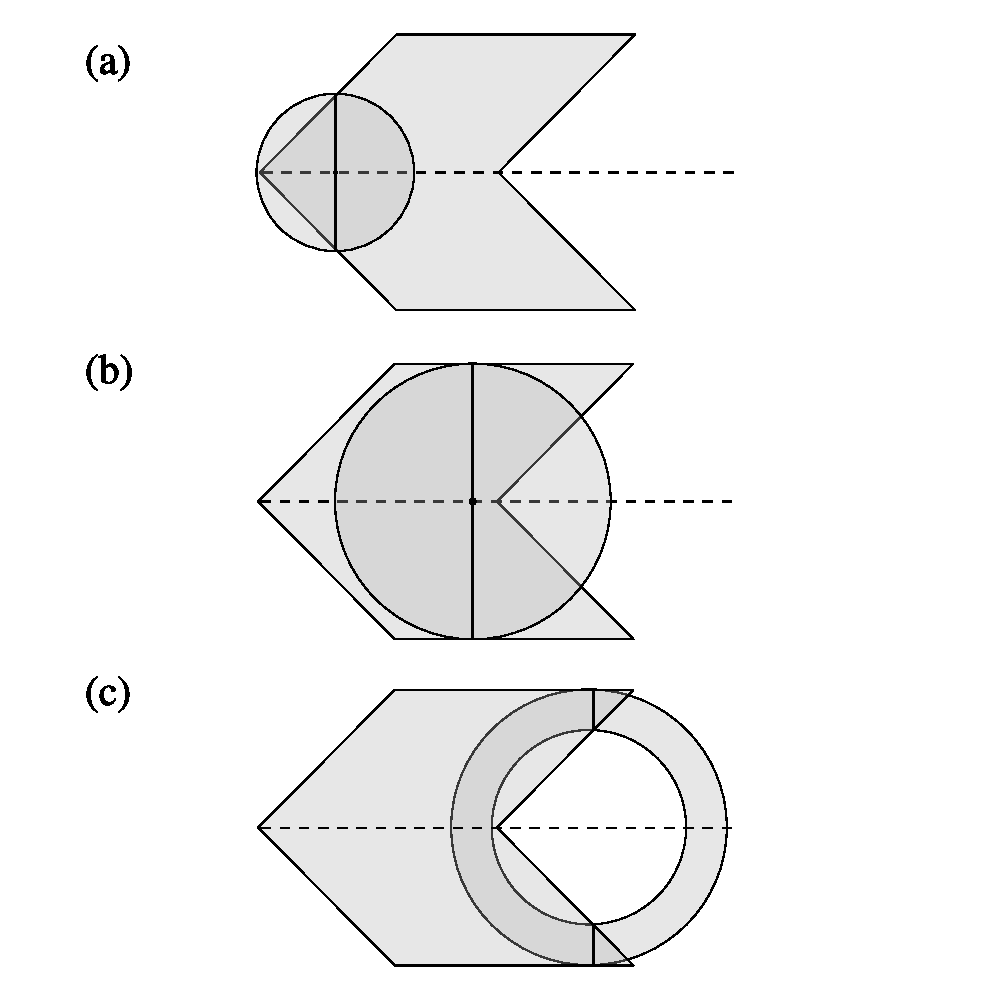
\includegraphics[width=0.5\textwidth]{growingsphere.pdf}
   \caption{Schematic representation of the growing communicating
   sphere, over the space--time diagrams, where time is represented on
   the horizontal direction, and space is represented in the vertical
   direction.  In (a) the sphere is
   growing as the surface of first contact has not reached the maximum
   distance.  In (b) it has reached the maximum distance, so that it
   remains at the same size.  After a Doomsday event, the signals can
   still be observed, but the surface of last contact grows }
   \label{F_sphere}
\end{figure}

  


\ack[Acknowledgement]{
%
This work was partially supported by the Consejo Nacional de
Investigaciones Cient\'{\i}ficas y T\'ecnicas (CONICET, Argentina),
the Secretar\'{\i}a de Ciencia y Tecnolog\'{\i}a, Universidad Nacional
de C\'ordoba, Argentina, and the Universidad Católica de Córdoba,
Argentina.
%
This research has made use of NASA's Astrophysics Data System.
%
Plots and simulations were made with software developed by the authors
using R and python languajes, plots were postprocessed with inkscape.
%
}


\bibliographystyle{mn2e}
\bibliography{biblio_seti}

\end{document}
